\documentclass[journal]{IEEEtran}
\usepackage[a5paper, margin=10mm, onecolumn]{geometry}
\usepackage[cmex10]{amsmath}
\usepackage{amssymb,amsfonts,amsthm}
\usepackage{gvv-book}
\usepackage{gvv}
\usepackage{hyperref}

\begin{document}


\title{2.8.6}
\author{EE25BTECH11025 - Ganachari Vishwambhar}
\maketitle

\textbf{Question}:\newline
Assuming that the straight lines work as the plane mirror for a point, find the image of the point $\brak{1,2}$ in the line $x-3y+4=0$.\\
\textbf{Solution: }\\
Translating the system by $\vec{A}=\myvec{4\\0}$ so that the line passes through origin:
\begin{align}
    L=\myvec{1&-3}\myvec{x\\y}=-4;
    \vec{P}=\myvec{1\\2}\\
    \vec{P}_{trans}=\vec{P}-\vec{A}=\myvec{1\\2}-\myvec{-4\\0}=\myvec{5\\2}\\
    L_{trans}=\myvec{1&-3}\myvec{x\\y}=0
\end{align}

Finding the normal vector:
\begin{align}
    \vec{N}=\myvec{1&-3}
\end{align}

Finding the unit normal vector:
\begin{align}
    ||\vec{N}||=\sqrt{1^2+\brak{-3}^2}=\sqrt{10}\\
    \vec{n}=\frac{\vec{N}}{||\vec{N}||}=\frac{1}{\sqrt{10}}\myvec{1\\-3}
\end{align}

Calculating the reflection matrix $R$ is given by the formula $R=I-2\vec{n}\vec{n}^T$
\begin{align}
    R=\myvec{1&0\\0&1}-2\brak{\frac{1}{\sqrt{10}}\myvec{1\\-3}}\brak{\frac{1}{\sqrt{10}}\myvec{1&-3}}
    =\myvec{\frac{4}{5}&\frac{3}{5}\\ \frac{3}{5}&\frac{-4}{5}}
\end{align}


Reflecting the given point:
\begin{align}
    \vec{P'}_{trans}=R.P_{trans}=\myvec{\frac{26}{5}\\ \frac{7}{5}}
\end{align}

Inverting the translation:
\begin{align}
    \vec{P'}=\vec{P'}_{trans}+\vec{A}=\myvec{\frac{6}{5}\\ \frac{7}{5}}
\end{align}

Thus the final image of the given point is $\vec{P'}=\myvec{\frac{6}{5}\\ \frac{7}{5}}$

\begin{figure}[h!]
   \centering
   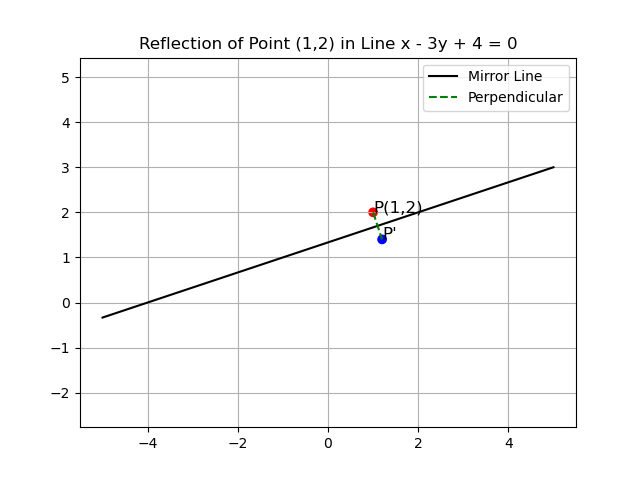
\includegraphics[width=0.7\linewidth]{figs/plot.png}
   \caption{Plot of the given line, point and reflected point}
   \label{}
\end{figure}
\end{document}  